%%%%%%%%%%%%%%%%%%%%%%%%
%
% $Autor: Hemanth Jadiswami Prabhakaran $
% $Datum: 2026-09-17 $
% $Pfad: GitHub/MBIDA_Thesis/report/Contents/General/en/10ApplicationAppendix.tex $
% $Version: 2 $
%
% $Project: MBIDA Thesis $
%
%%%%%%%%%%%%%%%%%%%%%%%%

\chapter{Appendix}
\label{chap:appendix}

This chapter supports the results in Chapter~\ref{chap:evaluation} without repeating them: Section~\ref{sec:fullSmapeTables} gives the complete sMAPE tables that Chapter~\ref{chap:evaluation}'s by-level and by-volume-segment comparisons are drawn from, covering every base-model/reconciler combination rather than only the figures needed to make a specific point there. Section~\ref{sec:fullCodeListings} then reproduces the artifacts this thesis is built on in full: the two notebooks (\texttt{01\_eda.ipynb} and \texttt{02\_pipeline.ipynb}), \texttt{config.py}, the Streamlit dashboard, and the two separate requirements files -- one for the pipeline environment, one for Streamlit Cloud deployment.

\section{Full sMAPE Tables}
\label{sec:fullSmapeTables}

The tables below report test-period sMAPE for all nine base-model/reconciler combinations produced by the pipeline (\texttt{02\_pipeline.ipynb}, reproduced in full in Section~\ref{sec:pipelineListing}), grouped by base model for readability. Each table's ``Base'' column is the unreconciled forecast; ``Bottom-Up'', ``MinTrace'', and ``Top-Down'' are that same base model's forecast after the corresponding reconciliation method (Section~\ref{sec:reconciliationTheory}).

\subsection{By Hierarchy Level}
\label{sec:smapeByLevel}

Table~\ref{table:smapeLevelHistavg} through Table~\ref{table:smapeLevelTheta} report sMAPE at each of the six hierarchy levels defined in Section~\ref{sec:hierarchyConstruction}.
\begin{table}[H]
	\centering
	\caption{sMAPE (\%) by hierarchy level -- HistoricAverage}
	\label{table:smapeLevelHistavg}
	\begin{tabular}{l S[table-format=2.2] S[table-format=2.2] S[table-format=2.2] S[table-format=2.2]}
		\toprule
		\textbf{Level} & {\textbf{Base}} & {\textbf{Bottom-Up}} & {\textbf{MinTrace}} & {\textbf{Top-Down}} \\
		\midrule
		Total      &  6.58 &  6.58 &  6.58 &  6.58 \\
		State      &  6.85 &  6.85 &  6.85 &  6.85 \\
		Store      &  8.19 &  8.19 &  8.19 &  8.19 \\
		Category   & 11.32 & 11.32 & 11.32 & 11.32 \\
		Department & 13.07 & 13.07 & 13.07 & 13.07 \\
		Item       & 40.91 & 40.91 & 41.76 & 40.91 \\
		\bottomrule
	\end{tabular}
\end{table}

\begin{table}[H]
	\centering
	\caption{sMAPE (\%) by hierarchy level -- AutoETS}
	\label{table:smapeLevelEts}
	\begin{tabular}{l S[table-format=2.2] S[table-format=2.2] S[table-format=2.2] S[table-format=2.2]}
		\toprule
		\textbf{Level} & {\textbf{Base}} & {\textbf{Bottom-Up}} & {\textbf{MinTrace}} & {\textbf{Top-Down}} \\
		\midrule
		Total      &  5.53 &  3.94 &  5.19 &  5.53 \\
		State      &  4.88 &  3.97 &  5.11 &  5.88 \\
		Store      &  5.95 &  4.77 &  5.58 &  7.60 \\
		Category   &  7.31 &  6.22 &  7.19 & 10.63 \\
		Department &  7.88 &  7.91 &  8.00 & 12.38 \\
		Item       & 37.72 & 37.72 & 40.62 & 40.74 \\
		\bottomrule
	\end{tabular}
\end{table}

\begin{table}[H]
	\centering
	\caption{sMAPE (\%) by hierarchy level -- Theta}
	\label{table:smapeLevelTheta}
	\begin{tabular}{l S[table-format=2.2] S[table-format=2.2] S[table-format=2.2] S[table-format=2.2]}
		\toprule
		\textbf{Level} & {\textbf{Base}} & {\textbf{Bottom-Up}} & {\textbf{MinTrace}} & {\textbf{Top-Down}} \\
		\midrule
		Total      &  4.24 &  3.78 &  4.36 &  4.24 \\
		State      &  4.32 &  3.76 &  4.36 &  4.77 \\
		Store      &  5.35 &  4.86 &  5.25 &  6.97 \\
		Category   &  6.73 &  6.18 &  6.52 &  9.75 \\
		Department &  8.26 &  7.60 &  7.98 & 11.49 \\
		Item       & 36.32 & 36.32 & 39.24 & 40.54 \\
		\bottomrule
	\end{tabular}
\end{table}

\subsection{By Volume Segment}
\label{sec:smapeByVolume}

Table~\ref{table:smapeVolumeHistavg} through Table~\ref{table:smapeVolumeTheta} report sMAPE at the bottom (item $\times$ store) level only, pooled within each cumulative training-volume bucket defined in Section~\ref{sec:volumeFramework}. The series counts per bucket -- reproduced once here since they are identical across all three tables -- are 29 (top 5\%), 94 (top 10\%), 326 (top 20\%), 2{,}151 (top 50\%), 8{,}155 (top 80\%), and 30{,}240 (top 100\%, i.e.\ all bottom-level series), out of 30{,}240 total.

% Add to preamble if not present:
% \usepackage{makecell}

\begin{table}[H]
	\centering
	\small
	\setlength{\tabcolsep}{4pt}
	\caption{sMAPE (\%) by volume segment -- HistoricAverage}
	\label{table:smapeVolumeHistavg}
	\begin{tabular}{
			S[table-format=3.0]
			S[table-format=5.0, group-separator={,}]
			S[table-format=2.2]
			S[table-format=2.2]
			S[table-format=2.2]
			S[table-format=2.2]
		}
		\toprule
		{\makecell{\textbf{Top \% of}\\\textbf{volume}}} & 
		{\makecell{\textbf{$n$}\\\textbf{series}}} & 
		{\textbf{Base}} & 
		{\makecell{\textbf{Bottom-}\\\textbf{Up}}} & 
		{\textbf{MinTrace}} & 
		{\makecell{\textbf{Top-}\\\textbf{Down}}} \\
		\midrule
		5 &    29 & 16.61 & 16.61 & 16.61 & 16.61 \\
		10 &    94 & 22.51 & 22.51 & 22.51 & 22.51 \\
		20 &   326 & 27.89 & 27.89 & 27.89 & 27.89 \\
		50 &  2151 & 28.88 & 28.88 & 28.88 & 28.88 \\
		80 &  8155 & 29.68 & 29.68 & 29.68 & 29.68 \\
		100 & 30240 & 40.91 & 40.91 & 41.76 & 40.91 \\
		\bottomrule
	\end{tabular}
\end{table}

\begin{table}[H]
	\centering
	\small
	\setlength{\tabcolsep}{4pt}
	\caption{sMAPE (\%) by volume segment -- AutoETS}
	\label{table:smapeVolumeEts}
	\begin{tabular}{
			S[table-format=3.0]
			S[table-format=5.0, group-separator={,}]
			S[table-format=2.2]
			S[table-format=2.2]
			S[table-format=2.2]
			S[table-format=2.2]
		}
		\toprule
		{\makecell{\textbf{Top \% of}\\\textbf{volume}}} & 
		{\makecell{\textbf{$n$}\\\textbf{series}}} & 
		{\textbf{Base}} & 
		{\makecell{\textbf{Bottom-}\\\textbf{Up}}} & 
		{\textbf{MinTrace}} & 
		{\makecell{\textbf{Top-}\\\textbf{Down}}} \\
		\midrule
		5 &    29 & 22.97 & 22.97 & 23.03 & 16.98 \\
		10 &    94 & 29.88 & 29.88 & 30.05 & 22.91 \\
		20 &   326 & 33.43 & 33.43 & 33.69 & 28.14 \\
		50 &  2151 & 31.93 & 31.93 & 32.51 & 28.99 \\
		80 &  8155 & 31.84 & 31.84 & 32.55 & 29.69 \\
		100 & 30240 & 37.72 & 37.72 & 40.62 & 40.74 \\
		\bottomrule
	\end{tabular}
\end{table}

\begin{table}[H]
	\centering
	\small
	\setlength{\tabcolsep}{4pt}
	\caption{sMAPE (\%) by volume segment -- Theta}
	\label{table:smapeVolumeTheta}
	\begin{tabular}{
			S[table-format=3.0]
			S[table-format=5.0, group-separator={,}]
			S[table-format=2.2]
			S[table-format=2.2]
			S[table-format=2.2]
			S[table-format=2.2]
		}
		\toprule
		{\makecell{\textbf{Top \% of}\\\textbf{volume}}} & 
		{\makecell{\textbf{$n$}\\\textbf{series}}} & 
		{\textbf{Base}} & 
		{\makecell{\textbf{Bottom-}\\\textbf{Up}}} & 
		{\textbf{MinTrace}} & 
		{\makecell{\textbf{Top-}\\\textbf{Down}}} \\
		\midrule
		5 &    29 & 22.97 & 22.97 & 23.01 & 17.47 \\
		10 &    94 & 30.41 & 30.41 & 30.98 & 23.42 \\
		20 &   326 & 32.79 & 32.79 & 34.38 & 28.48 \\
		50 &  2151 & 31.04 & 31.04 & 32.85 & 29.16 \\
		80 &  8155 & 31.10 & 31.10 & 32.87 & 29.73 \\
		100 & 30240 & 36.32 & 36.32 & 39.24 & 40.54 \\
		\bottomrule
	\end{tabular}
\end{table}

Two things worth noting when reading these tables alongside Chapter~\ref{chap:evaluation}. First, the by-level tables use a macro-average (sMAPE computed per series, then averaged), while the by-volume-segment tables pool every row in a bucket before computing sMAPE (a micro-average); the two happen to coincide at the Item level / top 100\% row because the evaluation grid is perfectly balanced, but they are not the same statistic in general. Second, HistoricAverage's Base, Bottom-Up, and Top-Down columns are identical to two decimal places at every level and bucket -- expected, since HistoricAverage is already coherent before reconciliation and Top-Down never changes the Total root, both of which the pipeline's own sanity checks (Section~\ref{sec:pipelineListing}) confirm directly.

\section{Full Code Listings}
\label{sec:fullCodeListings}

The two notebooks below are reproduced as executed -- code, narrative, and output together -- exported directly from Jupyter, so what appears here is the actual run these results come from rather than a re-typeset version of it. \texttt{config.py}, the dashboard, and both requirements files follow as plain listings, included directly from \texttt{Code/}.

\subsection{EDA Notebook}
\label{sec:edaListing}

\texttt{01\_eda.ipynb} is the companion notebook referenced throughout Chapters~\ref{chap:methodology} and~\ref{chap:evaluation}; every cleanup decision justified there traces to the specific pipeline step it feeds.


\includepdf[
pages=-,
scale=0.9,
pagecommand={\pagestyle{headings}}
]{../Code/10ApplicationAppendix/01_eda.pdf}

\subsection{Pipeline Notebook}
\label{sec:pipelineListing}

\texttt{02\_pipeline.ipynb} produces the base forecasts, reconciled forecasts, and sMAPE tables reported in Section~\ref{sec:fullSmapeTables} and discussed in Chapter~\ref{chap:evaluation}.

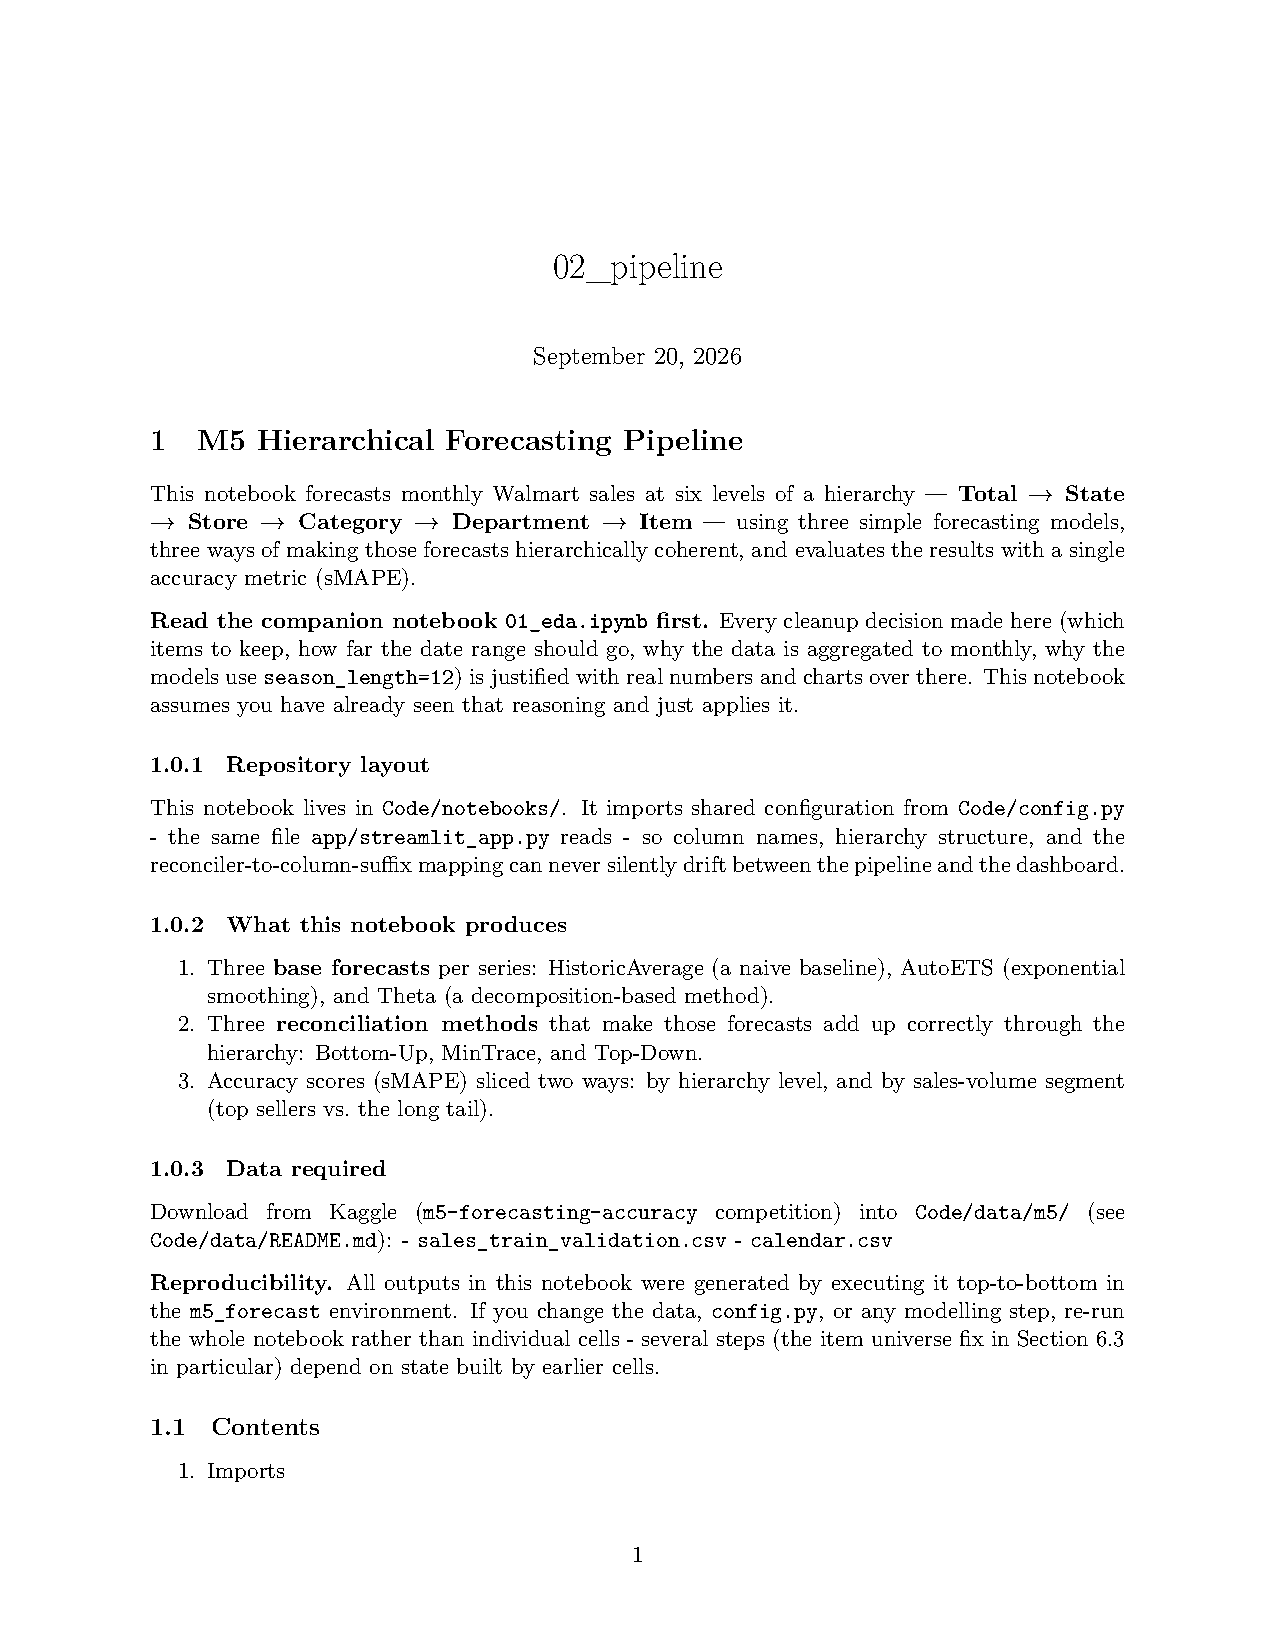
\includepdf[
pages=-,
scale=0.9,
pagecommand={\pagestyle{headings}}
]{../Code/10ApplicationAppendix/02_pipeline.pdf}

\subsection{\texttt{config.py}}
\label{sec:configListing}

The single shared configuration module read by both notebooks above and the Streamlit dashboard below, as introduced in Section~\ref{sec:configPy}.

\lstinputlisting[language=Python,style=pythonstyle,caption={Full code listing: \texttt{Code/config.py}}]{../Code/config.py}

\subsection{Streamlit Dashboard}
\label{sec:appListing}

The dashboard application described in Chapter~\ref{chap:appDeployment}, reading the four exported Parquet artifacts written by Section~16 of the pipeline notebook above.

\lstinputlisting[language=Python,style=pythonstyle,caption={Full code listing: \texttt{Code/app/streamlit\_app.py}}]{../Code/app/streamlit_app.py}

\subsection{Pipeline Requirements}
\label{sec:requirementsListing}

The full pinned dependency set used to execute both notebooks locally in the \texttt{m5\_forecast} environment.

\lstinputlisting[caption={Full listing: \texttt{Code/requirements-pipeline-raw.txt}}]{../Code/notebooks/requirements-pipeline-raw.txt}

\subsection{Deployment Requirements}
\label{sec:appRequirementsListing}

The separate, smaller requirements file that Streamlit Community Cloud actually installs when building the dashboard (Chapter~\ref{chap:appDeployment}) -- deliberately kept independent of the pipeline requirements above so that the deployed app is never held back by, or accidentally dependent on, packages only the notebooks need.

\lstinputlisting[caption={Full listing: \texttt{Code/app/requirements.txt}}]{../Code/app/requirements.txt}